
\newcommand{\PaperTitleHundrednm}{Effect of Augmented Collisional Ionization and potential depth in the VUV regime; a theoretical study}

\publication{\PaperTitleHundrednm}
\label{section:papers:100nm}

\begin{flushright}
Nicolas Bigaouette, Edward Ackad, Lora Ramunno\\
To be submitted
\end{flushright}

% Include PDF's abstract in the Table-of-Content as ``subsection 0'' but hide the number
\HidePDFAbstractNumber

\subsection{Author contributions}
The MD package was mostly written by N. B., as was the text. The ACI cross-sections were calculated
by E. A. All post processing scripts used to analyze data and generate figures
were written by N. B. Data generation and analysis was performed by N. B.
All authors contributed to the discussion.


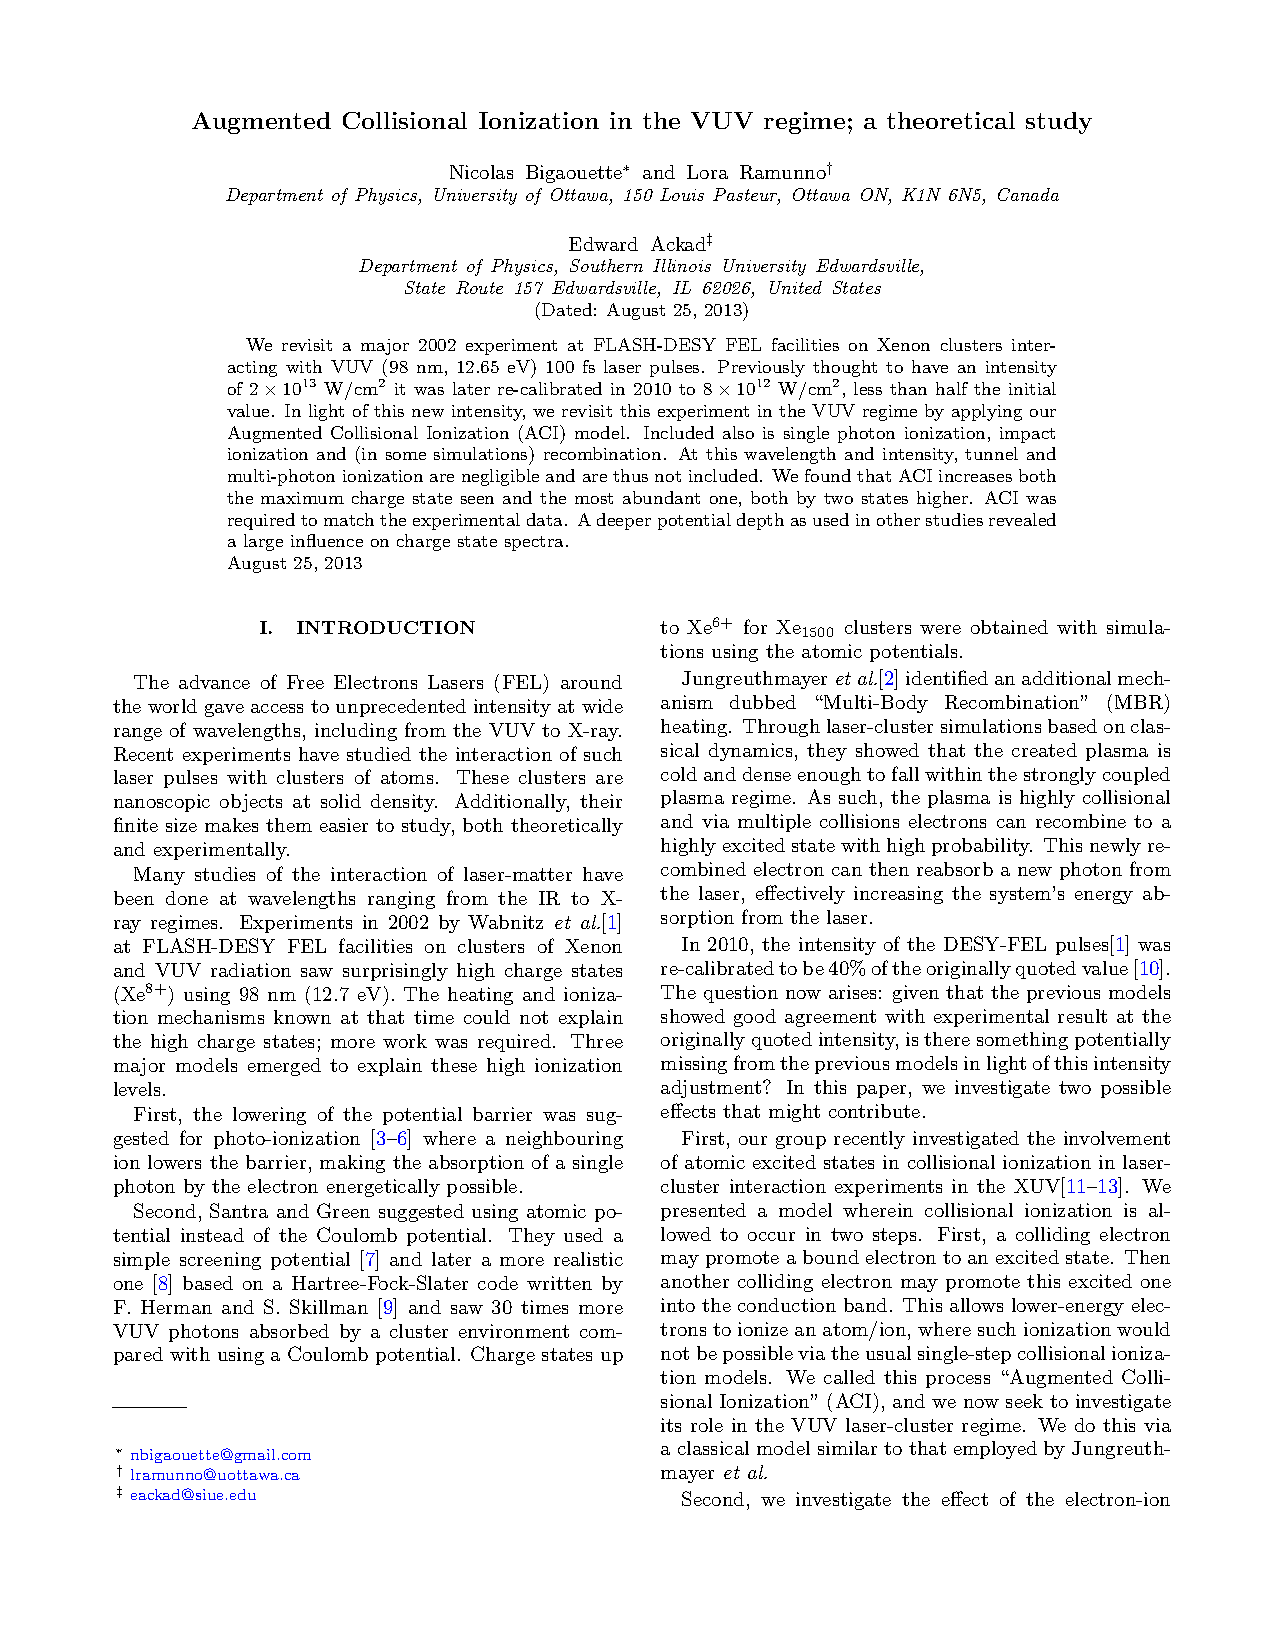
\includepdf[pages=-,
            addtotoc={
                % Original PDF page, TOC Section hierarchy, # matching TOC level, TOC label, \label{}
                % http://cs.brown.edu/system/software/latex/doc/pdfpages.pdf
                1,subsection,2,Abstract,paper_100nm_abstract,
                1,subsection,2,Introduction,paper_100nm_intro,
                2,subsection,2,Model,paper_100nm_model,
                2,subsubsection,3,Single photon ionization,paper_100nm_single,
                2,subsubsection,3,Threshold $V_p$,paper_100nm_thresh,
                2,subsubsection,3,Impact ionization,paper_100nm_impact,
                2,subsubsection,3,Augmented Collisional Ionization (ACI),paper_100nm_aci,
                3,subsubsection,3,Ground state recombination,paper_100nm_recomb,
                3,subsubsection,3,Many Body Recombination,paper_100nm_mbr,
                3,subsection,2,Results,paper_100nm_results,
                3,subsubsection,3,Effect of Augmented Collisional Ionization,paper_100nm_results_val,
                5,subsubsection,3,Effect of potential depth,paper_100nm_results_deeper,
                6,subsection,2,Conclusion,paper_100nm_results_conc,
                7,subsection,2,References,paper_100nm_results_refs
            }]{papers/Bigaouette2013_100nm.pdf}
